\chapter{Conhecendo as Progressives Web Apps}

\ac{PWA} é uma tecnologia emergente do Google, um conceito relativamente novo no mundo dos dispositivos móveis e da internet. De acordo com o Google Developers \cite{pwa}: \begin{citacao}
"As Progressive Web Apps fornecem uma experiência instalável, semelhante a um aplicativo, em computadores e dispositivos móveis que são criados e entregues diretamente pela Web. Eles são aplicativos da web que são rápidos e confiáveis. E o mais importante, são aplicativos da web que funcionam em qualquer navegador."
\end{citacao}

 \ac{PWA}s são desenvolvidas usando certas tecnologias e abordagens para criar aplicações que aproveitam os recursos dos dispositivos móveis nativos e de aplicativos da Web, essencialmente é uma mistura de aplicações web e mobiles nativas.

O Google definiu um \textit{checklist} a ser seguido para se considerar uma aplicação como uma \ac{PWA} são elas:

\begin{itemize}
	\item Progressivo - Funciona para qualquer usuário, independentemente do navegador escolhido, pois é criado com aprimoramento progressivo como princípio fundamental.
	\item Responsivo - Se adéqua a qualquer formato: desktop, celular ou tablet.
	\item Independente de conectividade - Aprimorado com \textit{service workers} para trabalhar \textit{off-line} ou em redes de baixa qualidade.
	\item Semelhante a aplicativos - Parece com aplicativos para os usuários, com interações e navegação de estilo de aplicativos, pois é compilado no modelo de \textit{shell} de aplicativo.
	\item Atual - Sempre atualizado graças ao processo de atualização do \textit{service worker}.
	\item Seguro - Fornecido via HTTPS para evitar invasões e garantir que o conteúdo não seja adulterado.
	\item Descobrível - Pode ser identificado como “aplicativo” graças aos manifestos W3C e ao escopo de registro do \textit{service worker}, que permitem que os mecanismos de pesquisa os encontrem.
	\item Reenvolvente - Facilita o reengajamento com recursos como notificações \textit{push}.
	\item Instalável - Permite que os usuários “guardem” os aplicativos mais úteis em suas telas iniciais sem precisar acessar uma loja de aplicativos.
	\item Linkável - Compartilhe facilmente por URL, não requer instalação complexa.
\end{itemize}

\section{Características}
\label{s_c4_caractetisticas}

\subsection{Confiável}
Quando iniciado a partir da tela inicial do usuário, os \textit{service workers} permitem que uma \ac{PWA} seja carregado instantaneamente, independentemente do estado da rede \cite{pwa}.


Basicamente os \textit{service workers} são \textit{scripts} que o navegador roda por debaixo dos panos, separado de uma página Web. Possibilitando que recursos sejam acessados mesmo sem uma interação do usuário ou de uma página Web. O \textit{service worker} possui hoje funcionalidades como \textit{Push Notifications}, que é basicamente, uma notificação que o usuário recebe sem requisita-lá, e Sincronização em Segundo Plano, que é uma \ac{API} que permite que a aplicação adie ações até que o usuário tenha uma conectividade com a internet estável. Isso é útil para garantir que uma ação feita pela o usuário, seja realmente realizada \cite{servicework} ???????????????.
O \textit{service worker} é uma \ac{API} interessante para os desenvolvedores já que permite configurar experiências off-line. Os S\textit{ervice Workers} possuem algumas características importantes:

\begin{itemize}
	\item É executado em uma \textit{thread} separada do navegador, portanto, não possui acesso ao \ac{DOM} diretamente.
	\item É um \textit{proxy} de rede programável, portanto, permite gerenciar as solicitações de rede da página.
	\item É encerrado quando ficar ocioso e reiniciado quando for necessário.
	\item Os \textit{service workers} utilizam promessas para retornar os dados de suas funções.
\end{itemize}

O \textit{Service Worker} possui um ciclo de vida à parte da página da Web e funciona em uma estrutura já determinada. Entendendo como cada evento ocorre e suas respostas é o ideal para se ter a melhor forma de atualizar e guardar os arquivos \cite{pwa2} ????. Primeiramente é necessário registrar o service worker na aplicação, isso pode ser feito via um arquivo \ac{JS}, pode se adicionar uma verificação, antes do registro, para verificar se o navegador suporta o uso de \textit{service worker}, após registrar o \textit{service worker} o navegador inicia a etapa de instalação em segundo plano ??????????.

Na etapa de instalação, é onde se normalmente é armazenado recursos estáticos em cache. Se todos os recursos forem salvos em cache corretamente, o service worker estará instalado. Se no momento de guardar os recursos, ocorrer alguma falha, a etapa de instalação não será finalizada corretamente, e portanto, o service worker não será ativado. Finalizando a etapa de instalação, é iniciada a fase de ativação, é nesse evento onde se gerencia o cache da aplicação e deleta coisas antigas de versões anteriores \cite{servicework} ????????.

Após a etapa de ativação, o service worker gerenciará as páginas dentro do seu escopo, com exceção da página que registrou o service worker, onde ela só será controlada se for carregada novamente. Enquanto o service worker estiver controlando as páginas, ele poderá assumir dois estados: tratando de eventos de busca e mensagens que as páginas possam gerar, ou encerrado, para economizar memoria do dispositivo \cite{servicework}.


Abaixo 	a \autoref{f_c4_sw_ciclo} mostra uma versão minimalista do ciclo de vida do service worker, em sua primeira instalação.
\newpage
\begin{figure}[!htpb]
	\centering
	\caption{Ciclo de Vida do Service Worker}
	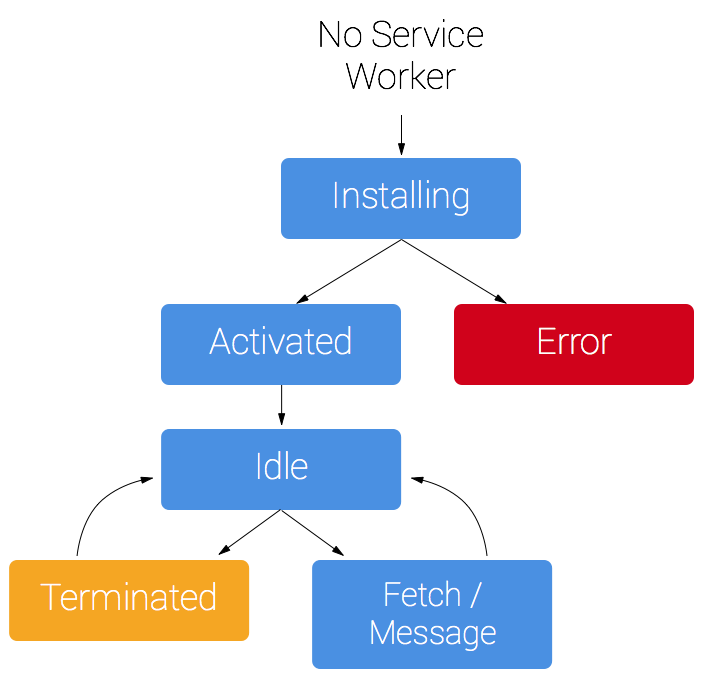
\includegraphics[width=7cm]{images/sw-lifecycle.png}\\
	Fonte:?????????????
 	\label{f_c4_sw_ciclo}
\end{figure}

\subsection{Rápido}
A maioria dos dados das \ac{PWA}s é salvo no armazenamento do dispositivo no primeiro acesso. A próxima vez que o usuário acessá-la, a aplicação fará o download de poucos dados. Este é um recurso útil para pessoas que possuem conexão com a internet limitada. O aplicativo é mais confiável do que apenas um site e permite que você envie notificações para seus usuários, mesmo depois que o aplicativo for fechado. Uma vez armazenado em um dispositivo, leva muito menos tempo para ser reativo do que um site comum que precisa buscar e carregar tudo de novo ???????????????.

\subsection{Integração e Engajamento}

As \ac{PWA}s são instaláveis e podem ser exibidos na tela inicial do usuário, sem a necessidade de uma loja de aplicativos, como Google Play Store ou Apple Store. Elas oferecem uma experiência imersiva em tela cheia com a ajuda do arquivo de manifesto do aplicativo web.

O Manifesto do Aplicativo Web, é um arquivo no formato \ac{JSON}, que permite controlar como a aplicação irá aparecer e como ela será iniciada, ela conterá também informações relevantes a aplicação, assim fazendo com que o navegador entenda que a aplicação é uma \ac{PWA} e assim o navegador apresentará uma mensagem para o usuário para que se possa instalar o app na tela inicial do \textit{smartphone} \cite{manifest}.

\begin{figure}[!htpb]
	\centering
	\caption{Adicionar a tela inicial}
	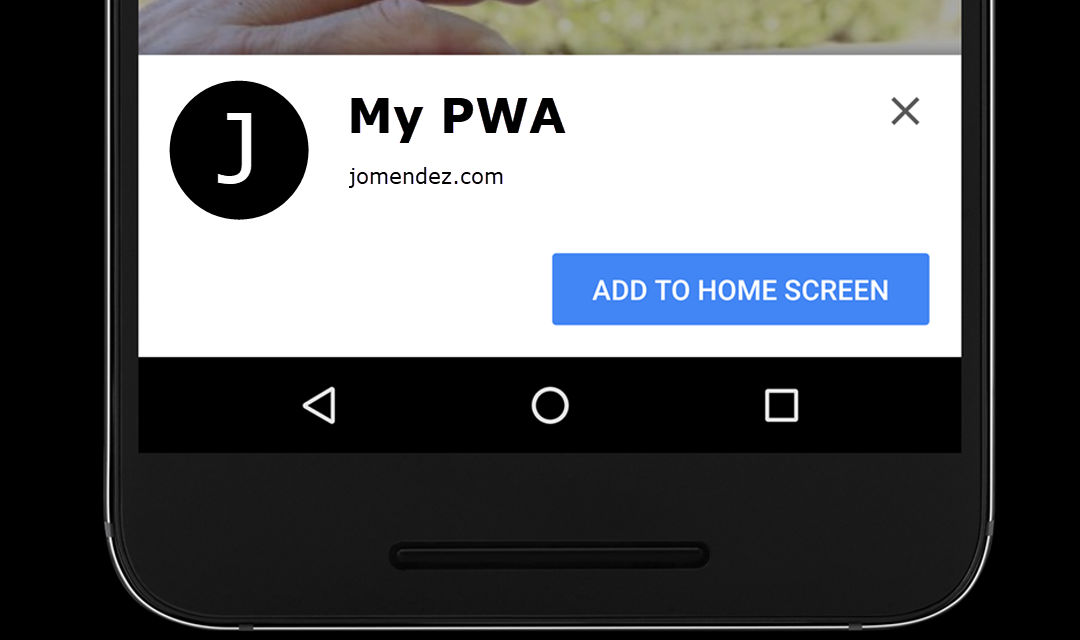
\includegraphics[width=12cm]{images/add-to-home-screen.png}\\
    Fonte:????????????????
 	\label{f_c4_add_home}
\end{figure}

Existem algumas configurações disponíveis no arquivo de manifesto, sendo algumas bem importantes como:

\begin{itemize}
	\item background color - Define a cor de fundo esperada para a aplicação. Esse valor repete o que já está disponível no CSS do site, mas pode ser usado pelos navegadores para desenhar a cor de fundo de um atalho quando o manifesto está disponível antes de a folha de estilo ser carregada. Isso cria uma transição suave entre o carregamento da aplicação e o carregamento do conteúdo do site \cite{manifestfile}.
	\item description - Fornece uma descrição geral do que a aplicação representa
	\item lang - Especifica o idioma principal para as propriedades, "name" e "short name"
	\item dir - Especifica a direção do texto principal para os membros "name", "short name" e "description". Juntamente com o membro "lang", ajuda na exibição correta dos idiomas da direita para a esquerda \cite{manifestfile}.
	\item display - Define o modo de exibição da aplicação.
	\item icons - Especifica uma lista de arquivos de imagem que podem servir como ícones de aplicativo, configurando de acordo com a resolução de tela do dispositivo.
	\item related applications - Define uma lista de aplicativos nativos que podem ser instalados ou acessíveis via plataforma externa, como Google Play Store, esses aplicativos podem ser versões alternativas da aplicação \ac{PWA} \cite{manifestfile}.
	\item short name - Fornece um nome curto legível para o aplicativo. Isso é feito quando não há espaço suficiente para exibir o nome completo da aplicação, como as telas iniciais dos dispositivos.
	\item theme color - Define a cor do tema padrão para a aplicação. Isso às vezes afeta o modo como o sistema operacional o exibe.
\end{itemize}

\section{Vantagens}
\subsection{Fácil Instalação e Atualização}
Como já foi apresentado, para adicionar ou instalar uma aplicação \ac{PWA}, os usuários simplesmente precisam abrir seu site progressivo em um navegador em seu dispositivo móvel. Em algum momento, eles serão solicitados a adicionar o aplicativo em sua tela inicial, ou os usuários podem adicionar o próprio \ac{PWA} no menu do navegador. Bem simples em comparação a aplicativos nativos, em que o usuário necessita ir a uma plataforma de aplicativos e instalar \cite{pwabenefits}.

Quanto às atualizações, os usuários de aplicações \ac{PWA} não precisam atualizar seu aplicativo toda vez que for lançada uma nova versão, eles sempre terão o mais novo.

\subsection{Custos Reduzidos de Desenvolvimento e Suporte}
Não precisa criar uma solução diferente para cada plataforma, pois o mesmo \ac{PWA} funciona no \textit{Android} e no \textit{iOS} e cabe em qualquer dispositivo. Devido à atualização fácil e simultânea, existirá apenas uma versão do aplicativo circulando. O que significa que não se gastará custos extras suportando várias versões \cite{pwabenefits}.

\subsection{Rápido, Leve e Seguro}
Com o \ac{PWA} implementado, a aplicação pode ser carregada em poucos segundos, o que é possível graças aos dados armazenados em cache pelos. Sendo menores em tamanho do que os aplicativos móveis nativos, as \ac{PWA} são mais leves e eficientes e usam menos capacidade e dados do dispositivo. Ao mesmo tempo, eles fornecem uma experiência de usuário próxima à de um aplicativo nativo \textit{Service Workers}. Além disso todas as aplicações \ac{PWA} funcionam via HTTPS, o que significa segurança extra e nenhum acesso não autorizado aos dados \cite{pwa2} ??????????????.

\subsection{Não necessita de nenhuma loja de aplicativos}
Para publicar uma aplicativo nativo para dispositivo móvel é necessário enviá-lo para alguma loja de aplicativos, como, Google Play Store ou Apple Store, e que ainda vai passar por um processo de análise do aplicativo. Com uma \ac{PWA}, não há necessidade de aguardar o término do período de moderação e como já mencionado, para instalar a aplicação progressiva, os usuários só precisarão abrir o website e clicar em "Adicionar à tela inicial". Embora se comportando como um aplicativo nativo, a \ac{PWA} ainda seria uma página da Web, clicável e compartilhável, e também é indexada pelo Google \cite{pwabenefits}.

\subsection{Customizável}
Se o usuário estiver sem conexão e quiser acessar novas páginas que não foram guardadas em cache, a aplicação não irá travar, mas mostrará uma mensagem personalizada, como na \autoref{f_c4_pwa_custom}:

\newpage
\begin{figure}[!htpb]
	\centering
	\caption{Telas Customizadas}
	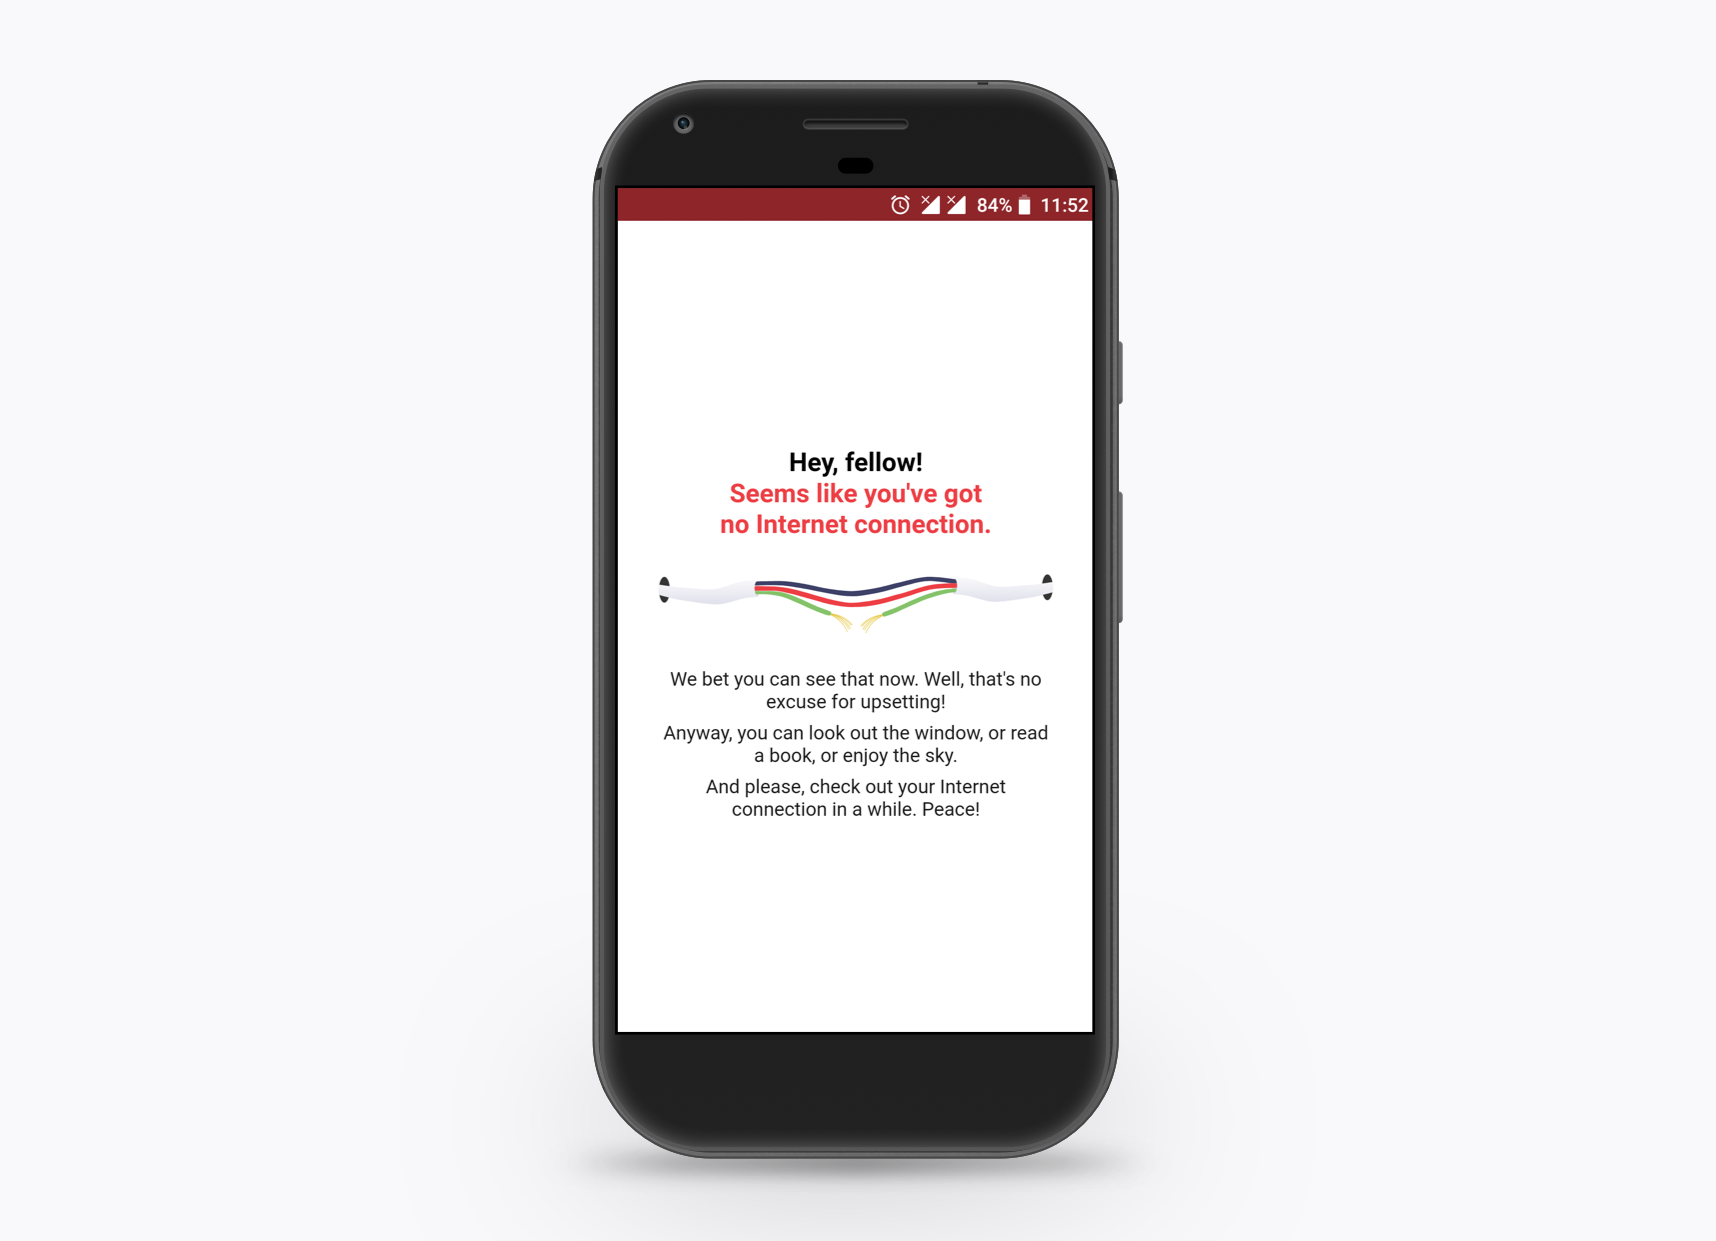
\includegraphics[width=13cm]{images/pwa_custom.png}\\
	Fonte:??????????
 	\label{f_c4_pwa_custom}
\end{figure}

\section{Desvantagens}
\subsection{Funcionalidades Limitadas}
As \ac{PWA}s ainda são sites e ainda não suportam todas as funcionalidades que os aplicativos nativos podem oferecer. Elas têm acesso limitado a recursos dos dispositivos. Além disso, as \ac{PWA}s podem oferecer um nível de notificação menos personalizado se comparado aos aplicativos nativos.

\subsection{Limitações para o iOS}
No momento, ainda há uma lacuna entre as \ac{PWA}s para Android e iOS. Embora os PWAs estejam disponíveis para usuários do iOS, nem todos os recursos que funcionam em dispositivos Android são oferecidos para iOS, no entanto, existe um movimento na equipe por trás do iOS que aos poucos estão implementando recursos para serem usados via \ac{PWA}, e provavelmente os usuários do iOS irão receber as mesmas funcionalidades das aplicações progressivas disponíveis no Android \cite{pwaios}.